\documentclass[tikz,border=8pt]{standalone}
% Shared look for every TikZ diagram. Load with \input{../../tools/tikz-style.tex}
\usepackage[T1]{fontenc}
\usepackage{lmodern}
\renewcommand{\sfdefault}{lmr}  % diagrams use the same serif as the text
\usetikzlibrary{arrows.meta, positioning, shapes.geometric, calc, fit, backgrounds}
\definecolor{cblue}{HTML}{4C78A8}
\definecolor{corange}{HTML}{F58518}
\definecolor{cgreen}{HTML}{54A24B}
\definecolor{cred}{HTML}{E45756}
\definecolor{cpurple}{HTML}{B279A2}
\definecolor{cgrey}{HTML}{6B6B6B}
\tikzset{
  every picture/.style={font=\sffamily, line width=1.2pt},
  box/.style={draw=#1, fill=#1!12, rounded corners=4pt, align=center, inner sep=7pt, minimum height=1.1cm},
  box/.default=cgrey,
  arrow/.style={-{Stealth[length=3mm]}, draw=cgrey, line width=1.4pt},
  title/.style={font=\sffamily\bfseries\Large},
  note/.style={font=\sffamily\small, text=cgrey, align=center},
}
\AtBeginDocument{\hyphenpenalty=10000 \exhyphenpenalty=10000}

% Section 8: the six steps of the template, with the Notebook's simulated income numbers.
\begin{document}
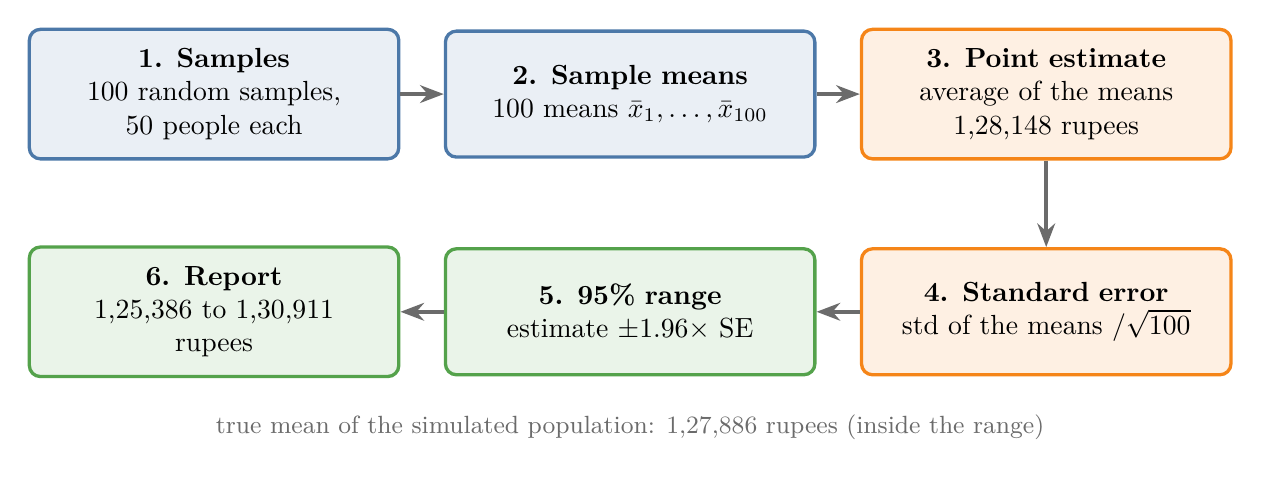
\begin{tikzpicture}[node distance=0.55cm]
  \tikzset{step/.style={box=#1, minimum width=4.6cm, minimum height=1.6cm, text width=4.2cm}}
  \node[step=cblue] (a) {\textbf{1. Samples}\\100 random samples,\\50 people each};
  \node[step=cblue, right=of a] (b) {\textbf{2. Sample means}\\100 means $\bar{x}_1, \dots, \bar{x}_{100}$};
  \node[step=corange, right=of b] (c) {\textbf{3. Point estimate}\\average of the means\\1,28,148 rupees};
  \node[step=corange, below=1.1cm of c] (d) {\textbf{4. Standard error}\\std of the means $/ \sqrt{100}$};
  \node[step=cgreen, left=of d] (e) {\textbf{5. 95\% range}\\estimate $\pm 1.96 \times$ SE};
  \node[step=cgreen, left=of e] (f) {\textbf{6. Report}\\1,25,386 to 1,30,911\\rupees};
  \draw[arrow] (a) -- (b); \draw[arrow] (b) -- (c); \draw[arrow] (c) -- (d);
  \draw[arrow] (d) -- (e); \draw[arrow] (e) -- (f);
  \node[note, below=0.35cm of e] {true mean of the simulated population: 1,27,886 rupees (inside the range)};
\end{tikzpicture}
\end{document}
